% =====================================================================
%  en-finance.tex  ·  A0 portrait academic poster (AFA / finance journal)
%  China Securities Index · Research
%  Compile with XeLaTeX (Palatino via newpxtext / newpxmath)
% =====================================================================
\documentclass[10pt]{article}

\usepackage[paperwidth=841mm,paperheight=1189mm,margin=0mm]{geometry}

\usepackage{fontspec}
\usepackage{newpxtext}
\usepackage{newpxmath}
\usepackage{amsmath}
\usepackage{booktabs,tabularx,array,colortbl}
\usepackage{tikz}
\usetikzlibrary{arrows.meta,calc,positioning}
\usepackage[most]{tcolorbox}
\usepackage{ragged2e}
\usepackage{xcolor}

% ---------------------------------------------------------------- palette
\definecolor{parchment}{HTML}{FBF8F2}
\definecolor{oxford}{HTML}{12263A}
\definecolor{burgundy}{HTML}{7A1F2B}
\definecolor{gold}{HTML}{A98B5F}
\definecolor{ink}{HTML}{1A1A1A}
\definecolor{stone}{HTML}{6B655C}

\pagecolor{parchment}
\color{ink}
\pagestyle{empty}
\setlength{\parindent}{0pt}
\setlength{\parskip}{3.8mm plus 0.5mm}
\setlength{\topskip}{0pt}
\setlength{\abovedisplayskip}{3.4mm plus 0.8mm minus 0.8mm}
\setlength{\belowdisplayskip}{3.4mm plus 0.8mm minus 0.8mm}
\setlength{\abovedisplayshortskip}{2.2mm}
\setlength{\belowdisplayshortskip}{2.2mm}
\setlength{\columnsep}{22mm}
\setlength{\emergencystretch}{3em}
\hyphenpenalty=800
\tolerance=2500
\raggedbottom

% ------------------------------------------------------------- type sizes
\renewcommand{\normalsize}{\fontsize{24}{31}\selectfont}
\renewcommand{\small}{\fontsize{21}{25}\selectfont}
\renewcommand{\footnotesize}{\fontsize{18}{22}\selectfont}
\renewcommand{\scriptsize}{\fontsize{16}{19}\selectfont}
\renewcommand{\large}{\fontsize{26}{31}\selectfont}
\renewcommand{\Large}{\fontsize{31}{36}\selectfont}
\renewcommand{\LARGE}{\fontsize{38}{44}\selectfont}
\renewcommand{\huge}{\fontsize{52}{58}\selectfont}
\renewcommand{\Huge}{\fontsize{80}{86}\selectfont}

% --------------------------------------------------------------- helpers
\newcommand{\kickerfont}{\fontsize{21}{25}\selectfont\addfontfeatures{LetterSpace=16}}
\newcommand{\sectnumfont}{\fontsize{33}{35}\selectfont\bfseries}
\newcommand{\secttitlefont}{\fontsize{31}{35}\selectfont\scshape\addfontfeatures{LetterSpace=6}}
\newcommand{\capfont}{\fontsize{20}{24}\selectfont}
\newcommand{\notefont}{\fontsize{16.5}{20}\selectfont}
\newcommand{\citex}[1]{\textsuperscript{\fontsize{14}{14}\selectfont[#1]}}
\newcommand{\status}[1]{{\fontsize{20}{24}\selectfont\color{stone}\textsc{Status.}\ #1\par}}
\DeclareMathOperator*{\argmin}{arg\,min}
\newcommand{\Vid}{V^{idx}}
\newcommand{\Pid}{P^{idx}}

% section heading: burgundy number, navy small-caps title, gold hairline
\newcommand{\postersection}[2]{%
  \par\vspace{10.2mm}%
  \noindent
  {\color{burgundy}\sectnumfont #1}\hspace{5mm}%
  {\color{oxford}\secttitlefont #2}\par
  \vspace{2.2mm}%
  {\color{gold}\rule{\linewidth}{0.55pt}}\par
  \vspace{3.4mm}%
}

% table caption above, figure caption below
\renewcommand{\arraystretch}{1.15}
\newcommand{\tabcaption}[2]{%
  \par\vspace{1mm}%
  {\capfont\color{oxford}\textsc{Table #1.}\ \itshape #2}\par
  \vspace{2.4mm}%
}
\newcommand{\figcaption}[2]{%
  \par\vspace{2.2mm}%
  {\capfont\color{ink}\hyphenpenalty=10000\relax
   \textbf{\textsc{Figure #1.}}\ #2}\par
}
\newcommand{\tabnote}[1]{%
  \par\vspace{1.6mm}%
  {\notefont\color{stone}\itshape #1}\par
}

% --------------------------------------------------------------- document
\begin{document}

% =====================================================================
% HEADER
% =====================================================================
\vspace*{14mm}
\noindent\hspace*{24mm}%
\begin{minipage}[t]{793mm}
{\color{gold}\rule{\linewidth}{1.1pt}}\par
\vspace{4.5mm}

\begin{minipage}[t]{450mm}
  {\kickerfont\color{burgundy}CHINA SECURITIES INDEX \textperiodcentered\ RESEARCH}\par
  \vspace{4mm}
  {\Huge\bfseries\color{oxford}Valuation without Ground Truth}\par
  \vspace{2.5mm}
  {\fontsize{37}{43}\selectfont\color{oxford}Bounded Multi-Agent Calibration for Index Constituents}\par
  \vspace{5.5mm}
  {\fontsize{27}{32}\selectfont\color{ink}%
    Yingzhou Chen\textsuperscript{\dag},\enspace
    Boyi Song\textsuperscript{\dag,$\ast$},\enspace
    Shenyi Sun\textsuperscript{\dag}}\par
  \vspace{3mm}
  {\fontsize{23}{27}\selectfont\color{ink}%
    China Securities Index Co., Ltd. (CSI), Shanghai, China}\par
  \vspace{2mm}
  {\fontsize{19}{23}\selectfont\color{stone}%
    \textsuperscript{\dag}Equal contribution.\enspace
    \textsuperscript{$\ast$}Corresponding author: Boyi Song, bysong@sse.com.cn}\par
\end{minipage}%
\hfill
\begin{minipage}[t]{318mm}\RaggedRight
  {\fontsize{20}{24}\selectfont\color{burgundy}\scshape\addfontfeatures{LetterSpace=8}Abstract}\par
  \vspace{2.4mm}
  {\fontsize{20}{25}\selectfont\color{ink}%
  Index levels aggregate prices, not values. We build the valuation counterpart:
  every constituent is valued by a hierarchical mixture of DCF, comparable and
  sentiment methods, routed by lifecycle, then aggregated with the same index
  weights. Because valuation has no ground truth, the system is never fitted to
  the index close. A bounded three-expert protocol updates a small parameter set
  under evidence gates and caps, formalized as a trust-region operator. Evidence
  covers five CSI indices and 2,201 constituents.}\par
\end{minipage}

\vspace{5mm}
{\color{gold}\rule{\linewidth}{0.4pt}}\par
\vspace{2.8mm}

% highlights
\begin{tcolorbox}[enhanced, colback=gold!6!parchment, colframe=gold!65!parchment,
  boxrule=0.4pt, arc=0mm, left=5mm, right=5mm, top=2.4mm, bottom=2.4mm, before skip=0mm, after skip=0mm]
\noindent
\begin{minipage}[c]{60mm}
  {\fontsize{18}{21}\selectfont\color{burgundy}\scshape\addfontfeatures{LetterSpace=10}Highlights}
\end{minipage}%
\hfill
\begin{minipage}[t]{221mm}\RaggedRight\hyphenpenalty=10000
  {\fontsize{20}{24}\selectfont\color{ink}%
  A valuation-implied index level, built from constituent values and index
  weights---not from prices.}
\end{minipage}%
\hfill
\begin{minipage}[t]{221mm}\RaggedRight\hyphenpenalty=10000
  {\fontsize{20}{24}\selectfont\color{ink}%
  Bounded expert review: evidence gates, severity caps, shadow/apply and
  baseline rollback.}
\end{minipage}%
\hfill
\begin{minipage}[t]{221mm}\RaggedRight\hyphenpenalty=10000
  {\fontsize{20}{24}\selectfont\color{ink}%
  No ground truth: synthetic benchmark, blind review and internal consistency;
  prices are diagnostic only.}
\end{minipage}
\end{tcolorbox}

\vspace{1.6mm}
{\color{gold}\rule{\linewidth}{1.1pt}}\par
\end{minipage}
\par\vspace{7mm}

% =====================================================================
% TWO COLUMNS
% =====================================================================
\noindent\hspace*{24mm}%
\begin{minipage}[t]{385.5mm}\RaggedRight

% ---------------------------------------------------------------------
\postersection{1}{Introduction}
An equity index is a weighted average of prices. It records what the market
pays, not what the constituents are worth. We construct the valuation
counterpart: value each constituent, then aggregate with the index weights.
The gap between the two levels shows where the index is rich or cheap relative
to fundamentals---a diagnostic, not a forecast, and never a target to fit.

Three fuzzinesses make this hard. \textit{Inputs} are fuzzy: reporting scope,
missing data, ST and newly listed firms, snapshots that are not fully
point-in-time. \textit{Models} are fuzzy: method applicability and lifecycle
classification. The \textit{objective} is fuzzy: there is no ground truth, and
price is not value. We therefore treat valuation as a conditional nonlinear
mapping and minimize process risk over a feasible parameter set, rather than
distance to the close.

\begin{tcolorbox}[enhanced, colback=white!35!parchment, colframe=white!35!parchment,
  boxrule=0pt, leftrule=1.8pt, arc=0mm, left=4mm, right=3mm, top=2.6mm, bottom=2.6mm]
{\fontsize{23}{28}\selectfont\color{oxford}\itshape
\textbf{\textsc{Research question.}} Can an index level be synthesized from
bounded, auditable valuation judgments---and can such a system be evaluated
when no ground truth exists?}
\end{tcolorbox}

\textbf{Four contributions.} (i) \textit{Problem}: threefold fuzziness, with no
price-as-label. (ii) \textit{Model}: a hierarchical mixture over lifecycle and
method, fuzzy aggregation, and index composition. (iii) \textit{Protocol}:
bounded three-expert review with gates, caps, shadow/apply and rollback,
formalized as a trust-region operator. (iv) \textit{Evidence}: five indices,
2,201 constituents, 170 regression tests, and an evaluation protocol that does
not need ground truth.

% ---------------------------------------------------------------------
\postersection{2}{Index Construction and Data}
Five indices, one market. Constituent weights are taken from published index
tables; the SSE Composite uses a full-market snapshot with total-market-cap
weights and the index's ST and seasoning rules\citex{6}. Financials are annual
reports, comparables are five same-industry firms, and sentiment is 30-day news
and forum text. All inputs are public; no paid data are used.

\tabcaption{1}{Five indices and the data used to value their constituents.}
{\fontsize{19}{24}\selectfont
\begin{tabularx}{\linewidth}{@{}>{\raggedright\arraybackslash}p{82mm}
  >{\raggedright\arraybackslash}p{40mm}
  >{\centering\arraybackslash}p{24mm}
  >{\raggedright\arraybackslash}X
  >{\raggedright\arraybackslash}p{86mm}@{}}
\arrayrulecolor{oxford}\toprule[1.2pt]
\rowcolor{white!55!parchment}
{\color{oxford}\textsc{Index}} & {\color{oxford}\textsc{Ticker}} &
{\color{oxford}\textsc{N}} & {\color{oxford}\textsc{Weight basis}} &
{\color{oxford}\textsc{Role}} \\
\arrayrulecolor{gold}\midrule[0.55pt]
SSE 50 & 000016.SH & 50 & Published cap weights & Large-cap blue chips \\
SSE 180 & 000010.SH & 180 & Published weights; float-cap fallback & Broad large-cap \\
STAR 50 & 000688.SH & 50 & Published weights & High-growth, loss-making \\
CSI 300 & 000300.SH & 300 & Published weights & Cross-market control \\
SSE Composite & 000001.SH & 2,201 & Total market capitalisation & All Shanghai A-shares \\
\arrayrulecolor{oxford}\bottomrule[1.2pt]
\end{tabularx}
}
\tabnote{Notes: $N$ is the number of constituents evaluated. The SSE Composite
excludes ST/*ST firms; new listings enter after one year (top ten by market
capitalisation after three months). Weights are used as published; a
weight-factor reconstruction is future work.}

% ---------------------------------------------------------------------
\postersection{3}{Valuation Framework}
Value is a conditional, nonlinear mapping. DCF needs cash-flow visibility;
comparables need a valid peer set; sentiment captures short-run pricing
pressure.\citex{4} Financials route to RIM/DDM, pre-revenue pharma to rNPV, and
multi-segment firms to SOTP. Lifecycle stage $z$ gates the method mix\citex{1},
so the same DCF parameters are not reused across young-growth and mature-stable
firms.

\begin{equation}
F(x;\Theta)=\sum_{z\in Z}p(z\mid x)\sum_{m\in M}w_{m\mid z}(x)\,f_{m,z}(x;\theta_{m,z})
\end{equation}
\begin{equation}
w_{m\mid z}(x)=\frac{a_m(x)\,\mu_{m,z}(x)\,e^{\gamma_m}}
{\sum_{j\in M}a_j(x)\,\mu_{j,z}(x)\,e^{\gamma_j}}
\end{equation}

Availability $a_m\in\{0,1\}$, applicability $\mu_{m,z}$, and a method prior
$e^{\gamma_m}$ set the conditional weights. Unavailable methods drop out and
the remainder renormalize.

\begin{equation}
\tilde{V}=\frac{\sum_m \tilde{w}_m\otimes\tilde{v}_m}{\sum_m\tilde{w}_m},
\qquad
[V]_\alpha=\Bigl\{\tfrac{\sum_m w_m v_m}{\sum_m w_m}:\ w_m\in[w_m]_\alpha,\ v_m\in[v_m]_\alpha\Bigr\}
\end{equation}
\status{Fuzzy weights are a proposed extension. The deployed engine uses crisp
weights with Monte Carlo and scenario intervals; the fuzzy layer and its
$\alpha$-cuts are not yet deployed.}

\begin{equation}
\Vid=\Pid\cdot\frac{\sum_i w_i\,(V_i/P_i)}{\sum_i w_i},
\qquad
V^{pw}=\Pid\cdot\frac{\sum_i w_iV_i}{\sum_i w_iP_i}
\end{equation}
The level scales by the weighted average relative valuation: if every stock is
valued at $k$ times its price, $\Vid=k\Pid$. Skipped names enter neither
numerator nor denominator. Price weighting is kept only as a control.

In economic terms, the gate allocates index valuation across methods according
to what each method can observe, and $\Vid/\Pid$ is the weighted average
value-to-price ratio---the index-level counterpart of a valuation multiple.

% ---------------------------------------------------------------------
% FIGURE 1 : two syntheses
\begin{center}
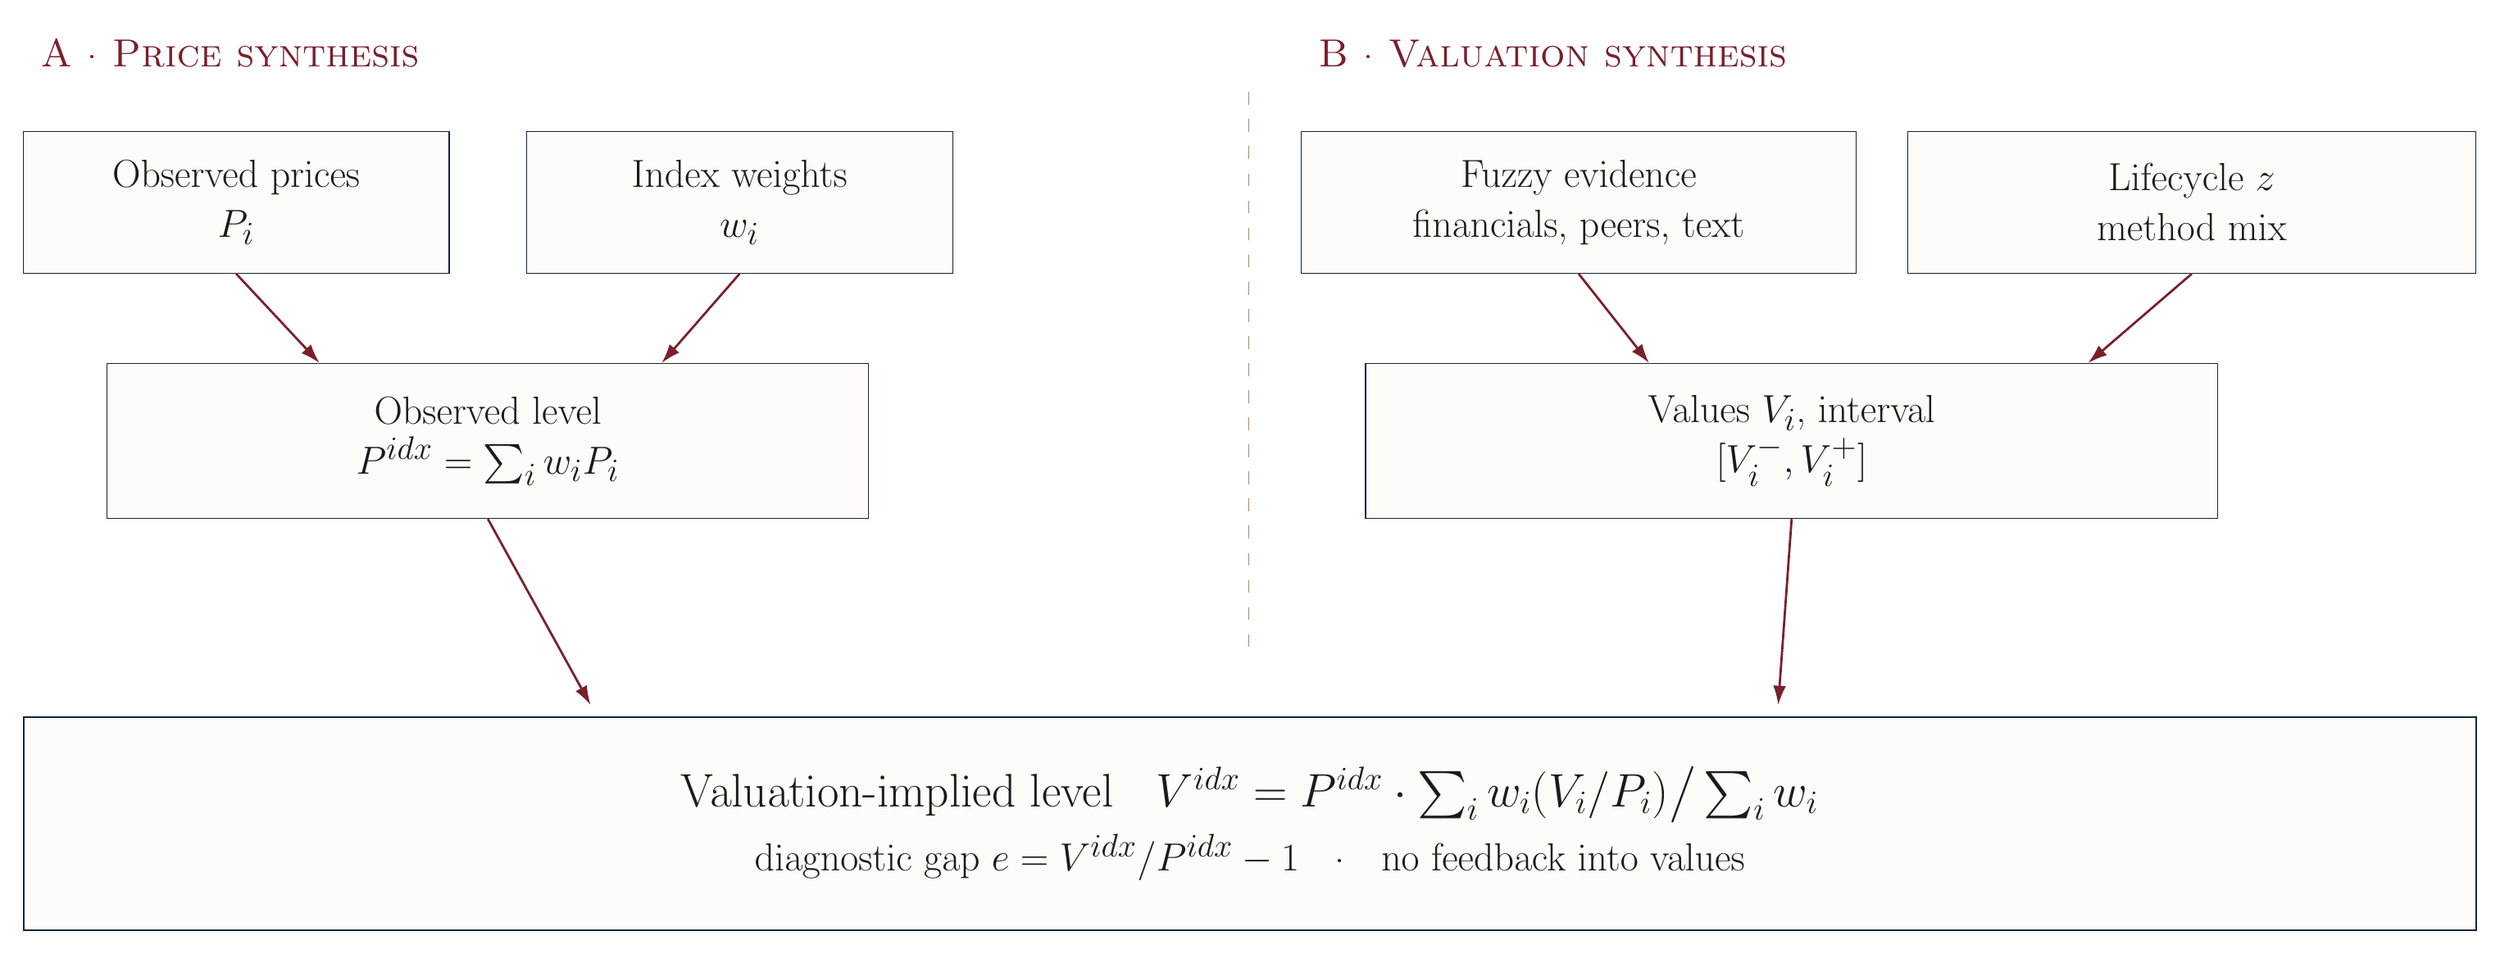
\begin{tikzpicture}[x=1mm,y=1mm,
  box/.style={draw=oxford, line width=0.45pt, fill=white!55!parchment,
    align=center, inner sep=2.2mm, font=\fontsize{19}{22}\selectfont, text=ink},
  arr/.style={-{Latex[length=3.0mm,width=2.0mm]}, draw=burgundy, line width=1.0pt},
  lab/.style={font=\fontsize{19}{22}\selectfont\scshape, text=burgundy, anchor=west}
]
\node[lab] at (0,140) {A \textperiodcentered\ Price synthesis};
\node[lab] at (198,140) {B \textperiodcentered\ Valuation synthesis};
\draw[gold, line width=0.4pt, dash pattern=on 2mm off 2.2mm] (190,48) -- (190,135);

\node[box, minimum width=66mm, minimum height=22mm, anchor=north west] (a1) at (0,128) {Observed prices\\$P_i$};
\node[box, minimum width=66mm, minimum height=22mm, anchor=north west] (a2) at (78,128) {Index weights\\$w_i$};
\node[box, minimum width=118mm, minimum height=24mm, anchor=north west] (a3) at (13,92) {Observed level\\$\Pid=\sum_i w_iP_i$};
\draw[arr] (a1.south) -- (46,92);
\draw[arr] (a2.south) -- (99,92);

\node[box, minimum width=86mm, minimum height=22mm, anchor=north west] (b1) at (198,128) {Fuzzy evidence\\financials, peers, text};
\node[box, minimum width=88mm, minimum height=22mm, anchor=north west] (b2) at (292,128) {Lifecycle $z$\\method mix};
\node[box, minimum width=132mm, minimum height=24mm, anchor=north west] (b3) at (208,92) {Values $V_i$, interval\\$[V_i^-,V_i^+]$};
\draw[arr] (b1.south) -- (252,92);
\draw[arr] (b2.south) -- (320,92);

\draw[arr] (a3.south) -- (88,39);
\draw[arr] (b3.south) -- (272,39);

\node[draw=oxford, line width=0.7pt, fill=white!55!parchment, align=center,
      inner sep=3mm, font=\fontsize{21}{25}\selectfont, text=ink,
      minimum width=380mm, minimum height=33mm, anchor=south west] (c) at (0,4) {%
  Valuation-implied level\quad $\Vid=\Pid\cdot\sum_i w_i(V_i/P_i)\big/\sum_i w_i$\\[1.2mm]
  {\fontsize{19}{23}\selectfont diagnostic gap $e=\Vid/\Pid-1$\quad\textperiodcentered\quad
  no feedback into values}};
\end{tikzpicture}
\end{center}
\figcaption{1}{Two syntheses of the same index. Price synthesis aggregates
observed prices; valuation synthesis aggregates model-implied values. The
implied level is anchored to the observed level and then compared as a
diagnostic---there is no feedback from the gap into the values.}

\end{minipage}%
\hspace{22mm}%
\begin{minipage}[t]{385.5mm}\RaggedRight

% ---------------------------------------------------------------------
\postersection{4}{Bounded Multi-Agent Calibration}
Review is bounded. Three domain experts---comparable quality, discount
parameters, sentiment---may propose only parameters in their own domain. A
chief reviewer accepts, clamps or rejects. Proposals must cite specific
evidence, clear a 0.65 confidence threshold, match severity to magnitude, and
stay inside hard caps: comparable 5/8/10 pp, sentiment 5/10 pp, WACC 0.4/1.0 pp,
terminal growth 0.2/0.6 pp. Changes are quantized on a fixed grid: 5 pp for
weights, 0.2 pp for WACC and growth.

Shadow mode records proposals without changing parameters; apply writes
accepted changes back, reruns the engine, and keeps a baseline for rollback.
Each batch snapshots its configuration.

\begin{equation}
\delta^\star=\argmin_{\delta\in\mathcal{C}}\ \mathcal{L}(\theta+\delta;e)+\lambda\lVert\delta\rVert_1,
\qquad
\mathcal{C}=\{\delta:\lvert\delta_j\rvert\le c_j(s),\ \theta+\delta\in\Theta_{\mathrm{feas}}\}
\end{equation}
Read as a trust region: sparse, severity-capped and feasible. The system does
not solve this program numerically; experts warm-start, and gates plus the chief
act as an approximate projection. Shadow is the counterfactual; apply is the
treatment.

% ---------------------------------------------------------------------
% FIGURE 2 : review protocol
\begin{center}
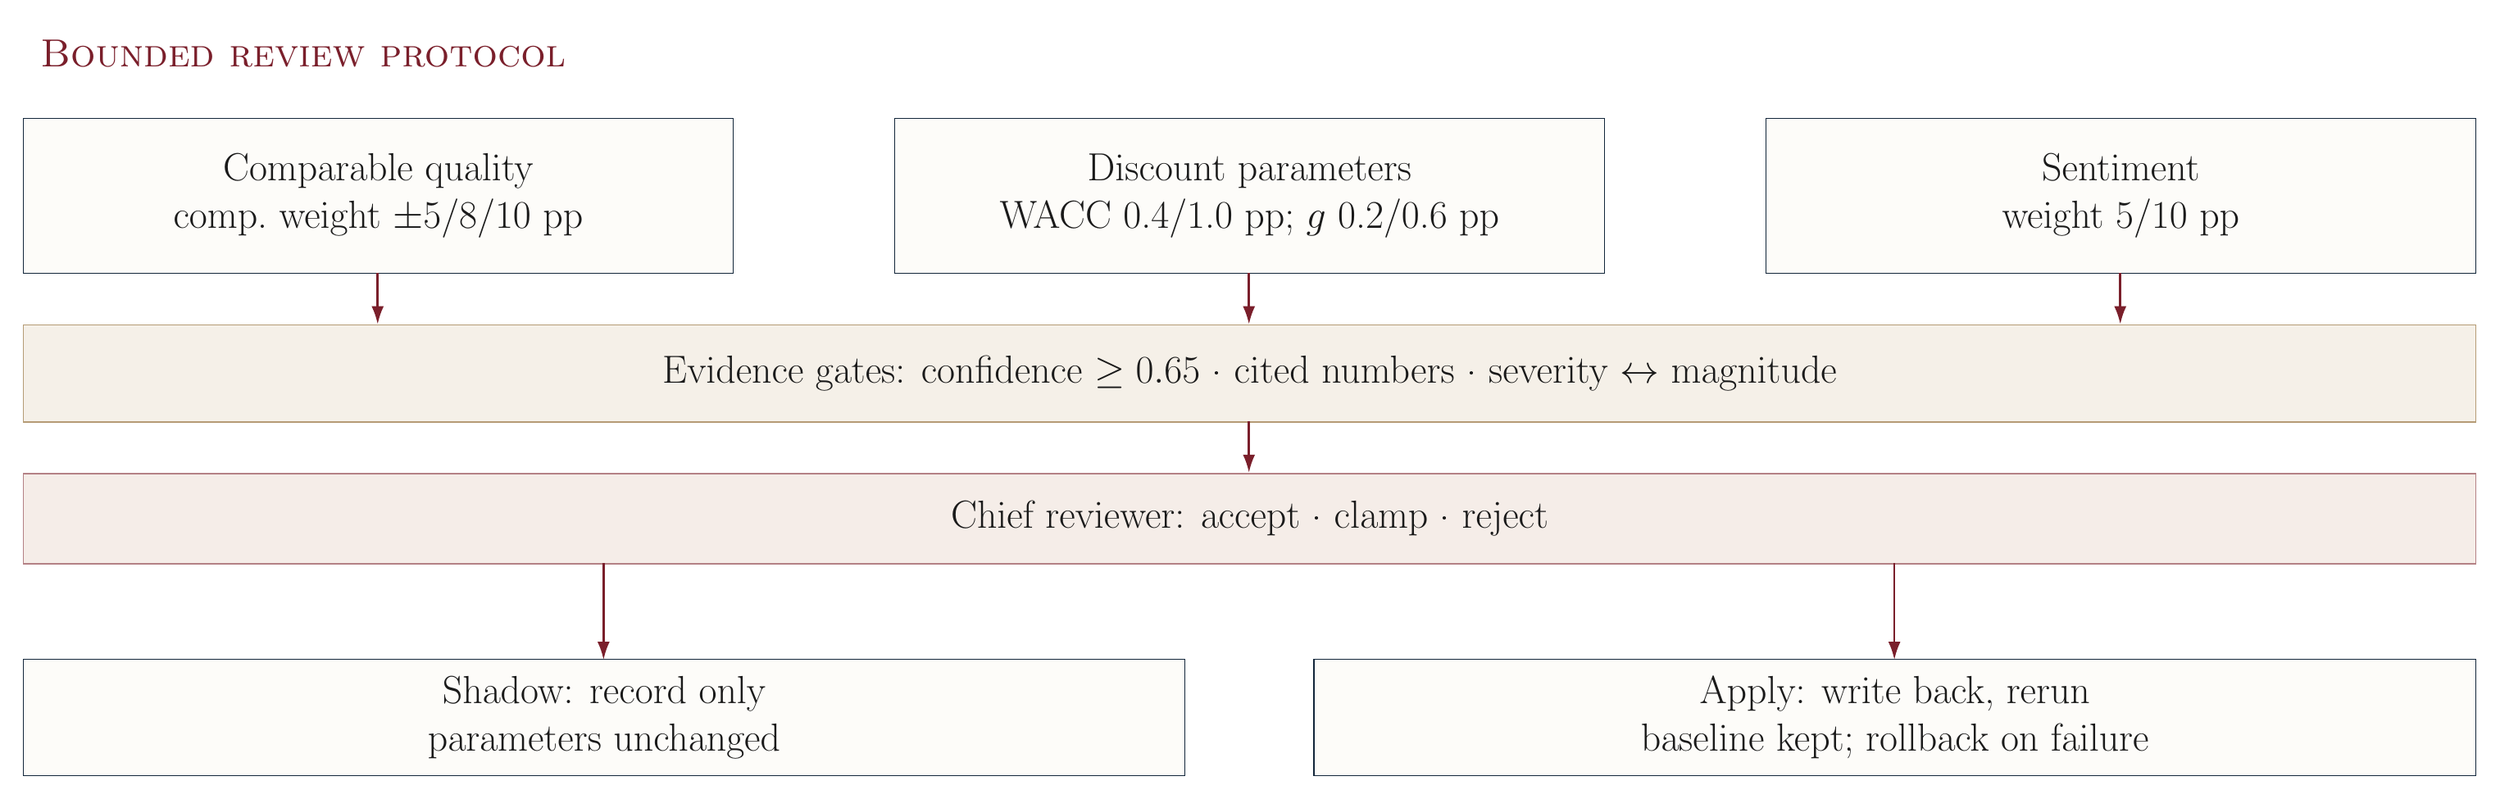
\begin{tikzpicture}[x=1mm,y=1mm,
  pbox/.style={draw=oxford, line width=0.45pt, fill=white!55!parchment,
    align=center, inner sep=2.0mm, font=\fontsize{18}{21}\selectfont, text=ink},
  band/.style={draw=gold!85!parchment, line width=0.6pt, fill=gold!7!parchment,
    align=center, inner sep=1.8mm, font=\fontsize{18}{22}\selectfont, text=ink},
  arr/.style={-{Latex[length=2.8mm,width=1.9mm]}, draw=burgundy, line width=0.95pt}
]
\node[font=\fontsize{19}{22}\selectfont\scshape, text=burgundy, anchor=west] at (0,114) {Bounded review protocol};

\node[pbox, minimum width=110mm, minimum height=24mm, anchor=north west] (e1) at (0,104) {Comparable quality\\{\fontsize{16}{19}\selectfont comp.\ weight $\pm$5/8/10 pp}};
\node[pbox, minimum width=110mm, minimum height=24mm, anchor=north west] (e2) at (135,104) {Discount parameters\\{\fontsize{16}{19}\selectfont WACC 0.4/1.0 pp; $g$ 0.2/0.6 pp}};
\node[pbox, minimum width=110mm, minimum height=24mm, anchor=north west] (e3) at (270,104) {Sentiment\\{\fontsize{16}{19}\selectfont weight 5/10 pp}};

\node[band, minimum width=380mm, minimum height=15mm, anchor=north west] (g) at (0,72) {Evidence gates: confidence $\ge 0.65$ \textperiodcentered\ cited numbers \textperiodcentered\ severity $\leftrightarrow$ magnitude};
\node[band, minimum width=380mm, minimum height=14mm, fill=burgundy!5!parchment,
      draw=burgundy!55!parchment, anchor=north west] (r) at (0,49) {Chief reviewer: accept \textperiodcentered\ clamp \textperiodcentered\ reject};

\node[pbox, minimum width=180mm, minimum height=18mm, anchor=south west] (sh) at (0,2) {Shadow: record only\\{\fontsize{16}{19}\selectfont parameters unchanged}};
\node[pbox, minimum width=180mm, minimum height=18mm, anchor=south west] (ap) at (200,2) {Apply: write back, rerun\\{\fontsize{16}{19}\selectfont baseline kept; rollback on failure}};

\draw[arr] (55,80) -- (55,72);
\draw[arr] (190,80) -- (190,72);
\draw[arr] (325,80) -- (325,72);
\draw[arr] (190,57) -- (190,49);
\draw[arr] (90,35) -- (90,20);
\draw[arr] (290,35) -- (290,20);
\end{tikzpicture}
\end{center}
\figcaption{2}{Bounded review protocol. Three domain experts propose capped
parameter changes; evidence gates filter them; the chief reviewer accepts,
clamps or rejects; shadow records, while apply writes back and can roll back to
the baseline.}

% ---------------------------------------------------------------------
\postersection{5}{Evaluation without Ground Truth}
No ground truth exists, so we evaluate the mechanism rather than the market.
(i) \textit{Synthetic benchmarks} with known values inject reporting errors,
missing comparables and routing errors. (ii) \textit{Blind review} by four to
six internal reviewers scores evidence, direction, magnitude and confidence over
two Delphi rounds with arbitration, reporting Krippendorff's $\alpha$.
(iii) \textit{Internal consistency} varies seeds, stock order and units, checks
shadow nullity and apply rollback, and runs eight automated report checks.

\tabcaption{2}{Metrics and their role. Only the final row uses market prices.}
{\fontsize{19}{24}\selectfont
\begin{tabularx}{\linewidth}{@{}>{\raggedright\arraybackslash}p{62mm}
  >{\raggedright\arraybackslash}X
  >{\raggedright\arraybackslash}p{92mm}@{}}
\arrayrulecolor{oxford}\toprule[1.2pt]
\rowcolor{white!55!parchment}
{\color{oxford}\textsc{Dimension}} & {\color{oxford}\textsc{Metric}} &
{\color{oxford}\textsc{Role}} \\
\arrayrulecolor{gold}\midrule[0.55pt]
Recovery & Relative error; interval coverage; routing accuracy & Synthetic benchmark \\
Calibration & ECE / Brier; confidence versus adoption & Expert judgment \\
Stability & Week-over-week $|\Delta\theta|$; seed dispersion & Process quality \\
Consistency & Shadow nullity; rollback; eight checks & Engineering \\
Market (diagnostic) & Direction hit rate; tracking error & Never optimised \\
\arrayrulecolor{oxford}\bottomrule[1.2pt]
\end{tabularx}
}
\tabnote{Notes: strictly proper scoring rules are used for calibration\citex{3}.
Market metrics are never used as an objective.}

Market prices appear only in the last row, as diagnostics. We make no accuracy
claim against the index level.

% ---------------------------------------------------------------------
\postersection{6}{Illustrative Evidence}
Table 3 collects the system's footprint and four shipped reference cases. They
show output format and scale; they are not an index-level backtest, and the
cases are selected, not randomly sampled.

\tabcaption{3}{System evidence and reference cases.}

{\fontsize{19}{24}\selectfont\color{oxford}\scshape\addfontfeatures{LetterSpace=7}Panel A \textperiodcentered\ System evidence}\par
\vspace{1.6mm}
\noindent
\begin{minipage}[t]{0.485\linewidth}
{\fontsize{18}{23}\selectfont
\begin{tabular*}{\linewidth}{@{}l@{\extracolsep{\fill}}r@{}}
\arrayrulecolor{oxford}\toprule[1.2pt]
Indices & 5 \\
Constituents & 2,201 \\
Shipped examples & 27 files \\
\arrayrulecolor{oxford}\bottomrule[1.2pt]
\end{tabular*}
}
\end{minipage}\hfill
\begin{minipage}[t]{0.485\linewidth}
{\fontsize{18}{23}\selectfont
\begin{tabular*}{\linewidth}{@{}l@{\extracolsep{\fill}}r@{}}
\arrayrulecolor{oxford}\toprule[1.2pt]
Regression tests & 170 \\
Report sections & 11 \\
Automated checks & 8 \\
\arrayrulecolor{oxford}\bottomrule[1.2pt]
\end{tabular*}
}
\end{minipage}

\vspace{3.2mm}
{\fontsize{19}{24}\selectfont\color{oxford}\scshape\addfontfeatures{LetterSpace=7}Panel B \textperiodcentered\ Reference cases (RMB 100 mn)}\par
\vspace{1.6mm}
{\fontsize{18}{23}\selectfont
\begin{tabularx}{\linewidth}{@{}>{\raggedright\arraybackslash}p{78mm}
  >{\raggedright\arraybackslash}X
  >{\raggedleft\arraybackslash}p{38mm}
  >{\raggedleft\arraybackslash}p{62mm}
  >{\raggedleft\arraybackslash}p{32mm}@{}}
\arrayrulecolor{oxford}\toprule[1.2pt]
Case & Sector & Central & Interval & Conf. \\
\arrayrulecolor{gold}\midrule[0.55pt]
Xinyao Microelectronics & AI chip design (fabless) & 271.23 & 149.81--423.03 & High \\
Changxin Technology & Semiconductors & 3,425.67 & 1,630.64--5,659.13 & High \\
Tianbo Intelligent & Auto thermal parts & 123.62 & 53.57--216.45 & High \\
Unitree Robotics & Humanoid / quadruped robots & 972.42 & 569.24--1,446.64 & High \\
\arrayrulecolor{oxford}\bottomrule[1.2pt]
\end{tabularx}
}
\tabnote{Notes: skill reference cases shipped with the examples; not an
index-level backtest; confidence is engine-reported and the examples are
selected, not a random sample.}

% ---------------------------------------------------------------------
\postersection{7}{Discussion}
\textbf{Implications.} A valuation-based level complements price indices: it
separates what is paid from what is earned, and decomposes the gap by
constituent, sector and method. For valuation research, estimation and
calibration stay apart---the engine produces values, agents propose bounded
parameter changes, and both leave an audit trail. For disclosure, the
configuration snapshot, per-constituent shadow record, eleven-section report and
eight checks make an algorithmic valuation reviewable \textit{ex post}.

\textbf{Limitations.} No ground truth, so validity rests on triangulation;
snapshots are not fully point-in-time; LLM proposals are stochastic
(temperature 0.1, no seed); public data are fragile. The fuzzy layer and
alternative pooling rules are proposed, not deployed.

\textbf{Next.} Point-in-time data, a cross-batch parameter ledger, damped gate
learning, external blind review, and out-of-sample index diagnostics.
Cross-market replication is the natural external-validity test.

\end{minipage}
\par

% =====================================================================
% REFERENCES + FOOTNOTE
% =====================================================================
\vfill
\noindent\hspace*{24mm}%
\begin{minipage}{793mm}
{\color{gold}\rule{\linewidth}{0.5pt}}\par
\vspace{2.6mm}
{\fontsize{20}{24}\selectfont\color{burgundy}\scshape\addfontfeatures{LetterSpace=8}References}\par
\vspace{2.2mm}
\begin{minipage}[t]{385.5mm}\RaggedRight
{\fontsize{18}{22}\selectfont\color{ink}
[1] Damodaran, A. (2012). \textit{Investment Valuation: Tools and Techniques
for Determining the Value of Any Asset}, 3rd ed. Hoboken: Wiley.\par
\vspace{1.2mm}
[2] Jacobs, R. A., Jordan, M. I., Nowlan, S. J., \& Hinton, G. E. (1991).
Adaptive mixtures of local experts. \textit{Neural Computation}, 3(1), 79--87.\par
\vspace{1.2mm}
[3] Gneiting, T., \& Raftery, A. E. (2007). Strictly proper scoring rules,
prediction, and estimation. \textit{Journal of the American Statistical
Association}, 102(477), 359--378.\par
}
\end{minipage}%
\hfill
\begin{minipage}[t]{385.5mm}\RaggedRight
{\fontsize{18}{22}\selectfont\color{ink}
[4] Baker, M., \& Wurgler, J. (2006). Investor sentiment and the cross-section
of stock returns. \textit{Journal of Finance}, 61(4), 1645--1680.\par
\vspace{1.2mm}
[5] Li, S., Yang, L., \& Wang, H. (2026). An LLM-based intelligent valuation
model for listed companies [in Chinese]. \textit{Securities Information
Technology}.\par
\vspace{1.2mm}
[6] Shanghai Stock Exchange (2020). \textit{SSE Composite Index Methodology}.
Shanghai.\par
}
\end{minipage}

\vspace{3.2mm}
{\color{gold}\rule{\linewidth}{0.4pt}}\par
\vspace{1.8mm}
{\notefont\color{stone}%
\textbf{\textsc{Not investment advice.}} Valuations are model outputs for
research and index diagnostics; they are not forecasts of index levels or
recommendations on any security. Reference cases are shipped examples, not an
index-level backtest.}\par
\end{minipage}
\par\vspace*{10mm}

\end{document}
